\chapter{Luminosity Measurement and Calibration}
\label{ch3}

Accurate measurement of the luminosity delivered to the CMS experiment by the LHC is essential for various reasons. Online, the luminosity measurement provides feedback on the LHC and CMS performance and operations, including measuring trigger rates. In offline analysis, the luminosity measurement is a critical component for measuring the cross-section of observed processes or setting upper limits in searches for processes beyond the standard model.

As we see, to measure luminosity, a total of seven luminometers are used at CMS, and each of them reads out a specific quantity observed in the detector, such as hits, tracks, or clusters. The rate R measured by the luminometer is proportional to the instantaneous luminosity, $\mathcal{L}_{inst}$, with the constant of proportionality given by the visible cross-section $\sigma_{vis}$ \cite{pas_18}.

\begin{equation}
R(t)=\mathcal{L}_{inst}\sigma_{vis}
\label{lumi_exp_gen}
\end{equation}

The determination of $\sigma_{vis}$ is performed through van der Meer (vdM) scans using a specialized LHC machine setup. This chapter provides a description of this procedure, specifically applied with the PCC method.


\section{Pixel Cluster Counting method}
\label{Pixel Cluster Counting method}

The PCC method is an offline technique that provides a luminosity measurement using the rate of pixel clusters. Due to the large area of the pixel detector and the relatively low occupancy of its sensors, the probability of a single pixel being struck by two charged particles from the same bunch crossing is extremely low. This high granularity and low occupancy result in an excellent linear response to pile-up (\(\mu\), the number of interactions per bunch crossing) \cite{PCC_PAS_12_001}. On average, the detector occupancy (# hit pixels/# total pixels) is less than 0.1\% \cite{lumi_precise_2015_2016}.  
Although the statistical precision per Lumisection (23-second period) is lower than that of online luminometers due to CMS trigger bandwidth limitations, PCC still provides a linear measurement with good precision over time. When integrated over longer periods, it delivers a stable and highly precise luminosity measurement.  

Figure \ref{pileup} shows a simulation with pp collision zero-bias events with the pixel cluster counting rate as a function of pileup in the pileup range observed in Run 2 from 0 to about 50 $\mu$. Where the mean number of pixel clusters is of the order of  111 per event. The red curve is a first-order polynomial fit with slope, the results indicate a high level of agreement, as evidenced by the estimated goodness-of-fit $\chi^{2}$ per degree of freedom (dof) of approximately 0.5, showing that the PCC rate is highly linear in this range under simulated conditions \cite{ Phase2_Upgrade,lumi_precise_2015_2016}.


\begin{center}
  \begin{figure}[h!]
    \centering
    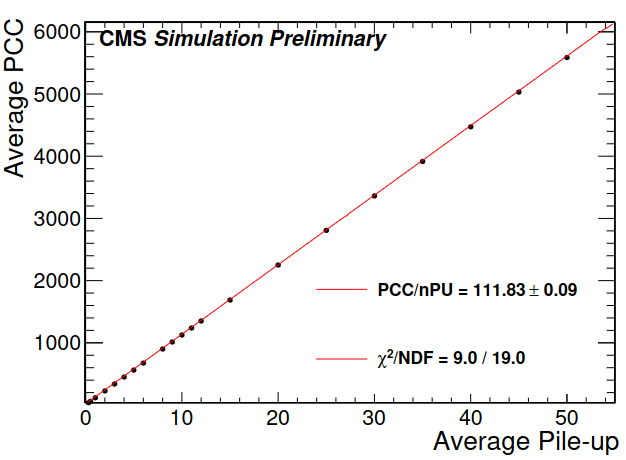
\includegraphics[scale=.35]{Chapter3/pileup_lineality.png} 
    \caption[PCC linearity with pile-up]{ Linearity of pixel cluster counting over the pileup range observed in Run 2 (from 0 to about 50) from simulation. The red line is a linear fit to the points \cite{Phase2_Upgrade} }
    \label{pileup}
  \end{figure}
\end{center}

For physics conditions, two data streams are recorded via the CMS DAQ: "zero-bias" and "random." The zero-bias stream consists of triggered data for colliding bunches at a bandwidth of approximately 2 kHz, while the random stream collects triggered data from all bunch crossings at a bandwidth of 500 Hz, primarily used for background estimation. The luminosity measurement is performed using the zero-bias data, whereas the random trigger helps evaluate background contributions.  

Under vdM conditions, a special trigger mode is employed to achieve higher data rates for PCC. This mode focuses on a selected set of five colliding bunch crossings, as detailed for each year in the next chapter, ensuring the necessary statistical precision.  

To derive the luminosity measurement from the PCC method, the mean number of pixel clusters per event is computed by averaging over several zero-bias events. This value is given by:

\begin{equation}
\left < N_{\text{cluster}} \right > \equiv \left < N_{\text{cluster}/\text{interaction}} \right > \mu
\end{equation}

Under minimum bias conditions, $\mu$ can be expressed as: 

\begin{equation}
\mu = \frac{\sigma_{\text{minBias}}}{f} \cdot \mathcal{L}_{inst}
\end{equation}

where $f$ is the LHC revolution frequency and $\mathcal{L}_{inst}$ is the single bunch instantaneous luminosity (SBIL). The minimum bias cross section $\sigma_{\text{minBias}}$ here is related to the PCC visible cross section by the mean number of clusters per interaction:

\begin{equation}
\sigma_{vis}= \left < N_{\text{cluster}/\text{interaction}} \right >\cdot \sigma_{\text{minBias}}
\end{equation}

Combining everything, the PCC luminosity measurement is obtained as:

\begin{equation}
\mathcal{L}_{inst}=\frac{\left < N_{\text{cluster}} \right> f}{\sigma_{vis}}
\end{equation}

In the PCC measurement, the innermost layer (Layer 0) of the pixel detector is excluded due to significant dynamic inefficiency effects. At high instantaneous luminosities, the hit efficiency decreases because the readout chip cannot process all hits in time.

For PCC rate measurements, only the pixel detector modules that remain stable throughout the entire data-taking period (year) are used. Modules known to be defective or significantly affected by the limited size of the readout buffer are excluded from the analysis.

The final number of excluded modules, referred to as "veto modules," is detailed for each year in the next chapter.

%This method is capable of providing a precise luminosity measurement over longer time periods, but it cannot do so for a single luminosity section (23 seconds) as is possible with online luminometers. The reason for this limitation is the limited CMS trigger bandwidth available for collecting data \cite{pas_18}. A detailed discussion on this topic can be found in the next chapter.\\

%PCC si calcula lumi por cada lumi section.  Esto no tiene que ver con online vs offline.  PCC es un offline luminometro, quiere decir que los datos llegan tarde.  Con PCC solo podemos calcular lumi cada lumi section, debido a la baja estadistica (por la lectura de los datos de zero bias).  otros luminometros tienen precision con NB4 (HF, PLT, BCM1F).  


\section{Luminosity calibration: van der Meer method}
\label{vdM method}

As discussed in Chapter 1, the instantaneous luminosity for a single colliding bunch is described by Eq. (\ref{luminosity_2}). In practice, while the measurement of the beam currents $N_{1,2}$ is well determined, the individual proton density functions cannot be directly measured. To address this, the vdM method involves a specific machine setup that allows for the determination of the two beam overlap integrals. This is achieved by varying the separation between the beams and measuring the resulting rates, which can be used to obtain density profiles that are close to normal distributions. The beam overlap can be expressed in terms of the measured rates as follows:

\begin{equation}
\int \rho_{x1}(x) \rho_{x2}(x) dx = \frac{R_{x}(0)}{\int R_{x}(\Delta) d\Delta}
\end{equation}

where $R_{x}(\Delta)$ is the rate measured when the two beams are separated in $x$ by a distance $\Delta$; a similar equation can be written in $y$. Then the beam overlap width $\Sigma_{x}$ (and similarly $\Sigma_{y}$) is defined as \cite{pas_18}:

\begin{equation}
\Sigma_{x}= \frac{1}{\sqrt{2\pi}} \frac{\int R_{x}(\Delta)d\Delta}{R_{x}(0)}
\label{CapSigma}
\end{equation}

This process leads to the final expression for luminosity for a single colliding bunch:

\begin{equation}
\mathcal{L}_{inst}=\frac{N_{1} N_{2}f}{2 \pi \Sigma_{x}\Sigma_{y}}
\end{equation}

where $N_{1,2}$ are the particles per bunch (bunch current) and  $f= 11246$ Hz is the bunch orbit frequency around the LHC ring determined by the energy of the protons.\\

Therefore, the equation ~\ref{lumi_exp_gen} used to measure the visible cross sections $\sigma_{vis}$ takes the following form:

\begin{equation}
  \sigma_{vis}=2\pi \frac{ R(0, 0)}{N_{1}N_{2} f} \Sigma_{x} \Sigma_{y}
  \label{sigmavis_eq}
\end{equation}

Experimentally, the quantities $\Sigma_{x}$ and $\Sigma_{y}$, as defined in Eq. (\ref{CapSigma}), are determined by conducting two separate scans in the $x$ and $y$ directions, respectively. 
These scans are performed by varying the separation between the beams in each direction  at a fixed number of separation steps.The separation steps are determined through curve fitting of the scan data based on the luminometer rate measurements obtained during the vdM scans.\\

The measured rate, denoted by $R(0,0)$, is determined as the average value among the rates obtained in the $x$-scan $R_x(0)$, and the rates obtained in the $y$-scan $R_y(0)$. Although the beam widths are identical for all luminometers, the peaks of the scan curves are specific for each luminometer.\\

Figure \ref{vdm_sketch} depicts a schematic of the beam positions during vdM scans in the $x$ and $y$ planes, along with the detector rate as a function of beam separation  \cite{pas_18}.
\newpage
\begin{center}
  \begin{figure}[ht]
    \centering
    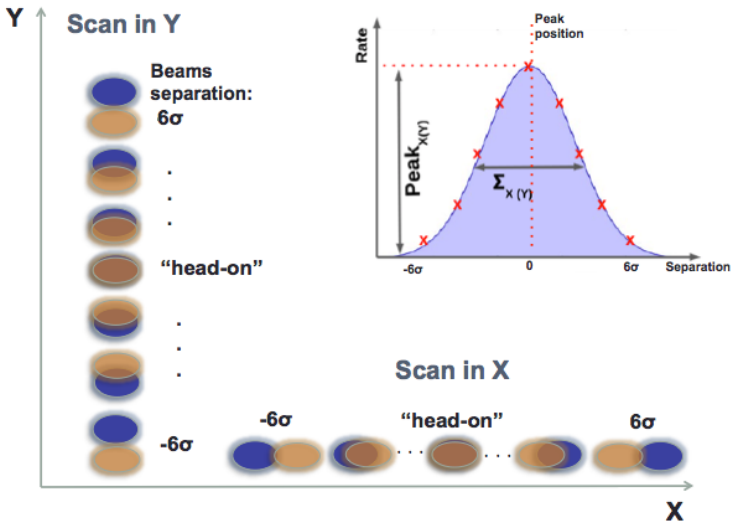
\includegraphics[scale=.50]{Chapter3/vdm_sketch.png}
    \caption[Sketch of a vdM scan in $x$ and $y$ directions and example of fitting resulting rates]{ The sketch of a vdM scan in $x$ and $y$ planes. The indent sketch is an example of the fit of the resulting rates \cite{vdM_sketch}.}
    \label{vdm_sketch}
  \end{figure}
\end{center}








\section{2017 and 2018 data Collected}
\label{Run 2 data Collected}

In June 2017, data collection for the second phase of Run 2 of the Large Hadron Collider (LHC) began, covering the years 2017 and 2018. As a result, a total recorded luminosity of \(49.81 \, \text{fb}^{-1}\) for 2017 and \(67.86 \, \text{fb}^{-1}\) for 2018 was achieved. This data was collected during proton-proton collisions at a center-of-mass energy of \(\sqrt{s} = 13\) TeV.  

The data-taking period started with the establishment of stable beams and ended either when the beam was intentionally stopped or when stable beams were temporarily interrupted for beam studies.  

Each year, a dedicated setup is allocated for the van der Meer (vdM) program, which will be discussed in a later chapter. This program is essential for the calibration of luminosity and the determination of its associated uncertainty, which plays a crucial role in the analyses where luminosity is a key factor.  

The luminosity delivered by the LHC to CMS (shown in blue) and the luminosity recorded by CMS (depicted in orange) during 2017 are illustrated in Figure~\ref{Lumi_2017}, while Figure~\ref{Lumi_2018} presents the corresponding data for 2018~\citep{wikicern}.



\begin{center}
  \begin{figure}[h!]
    \centering
    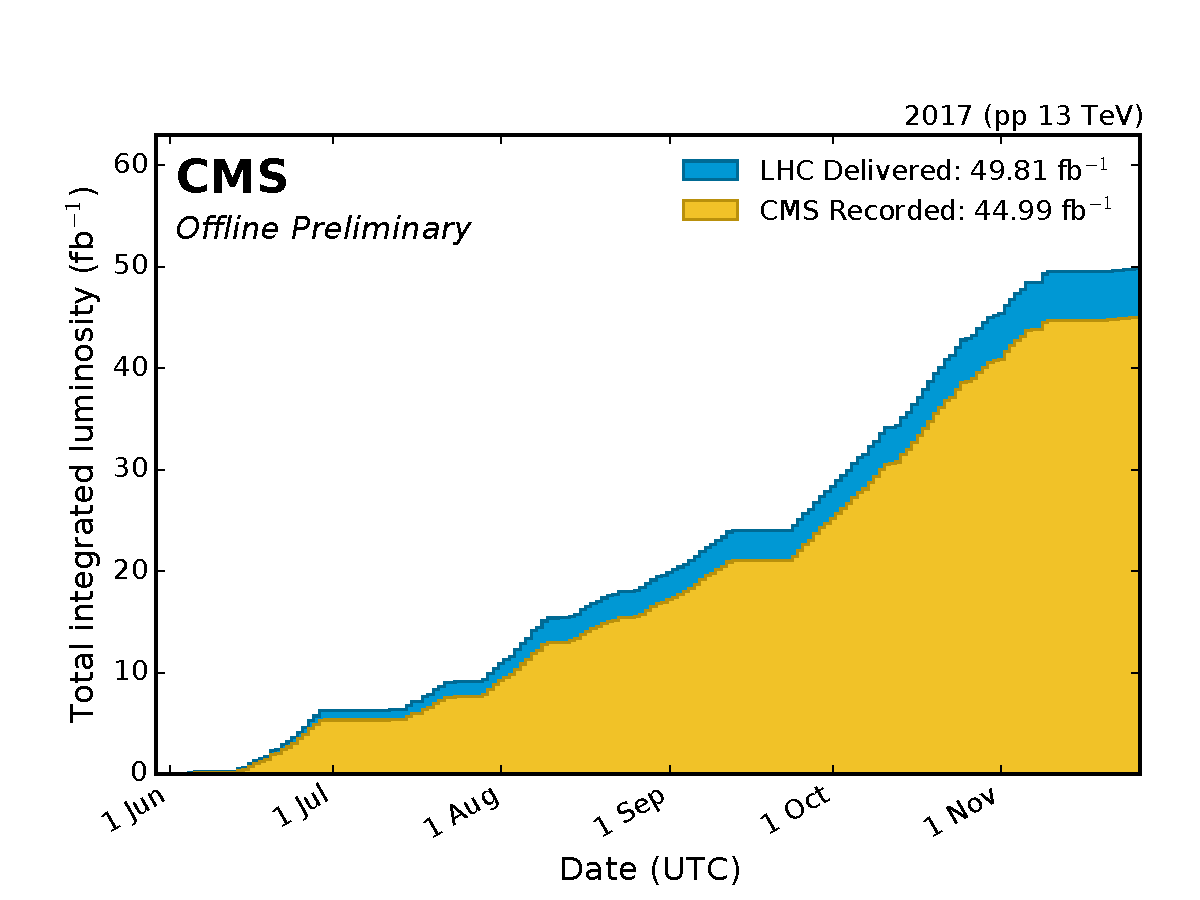
\includegraphics[width=.45\textwidth]{Chapter3/Luminosity/int_lumi_per_day_cumulative_pp_2017_Normtag.pdf}
    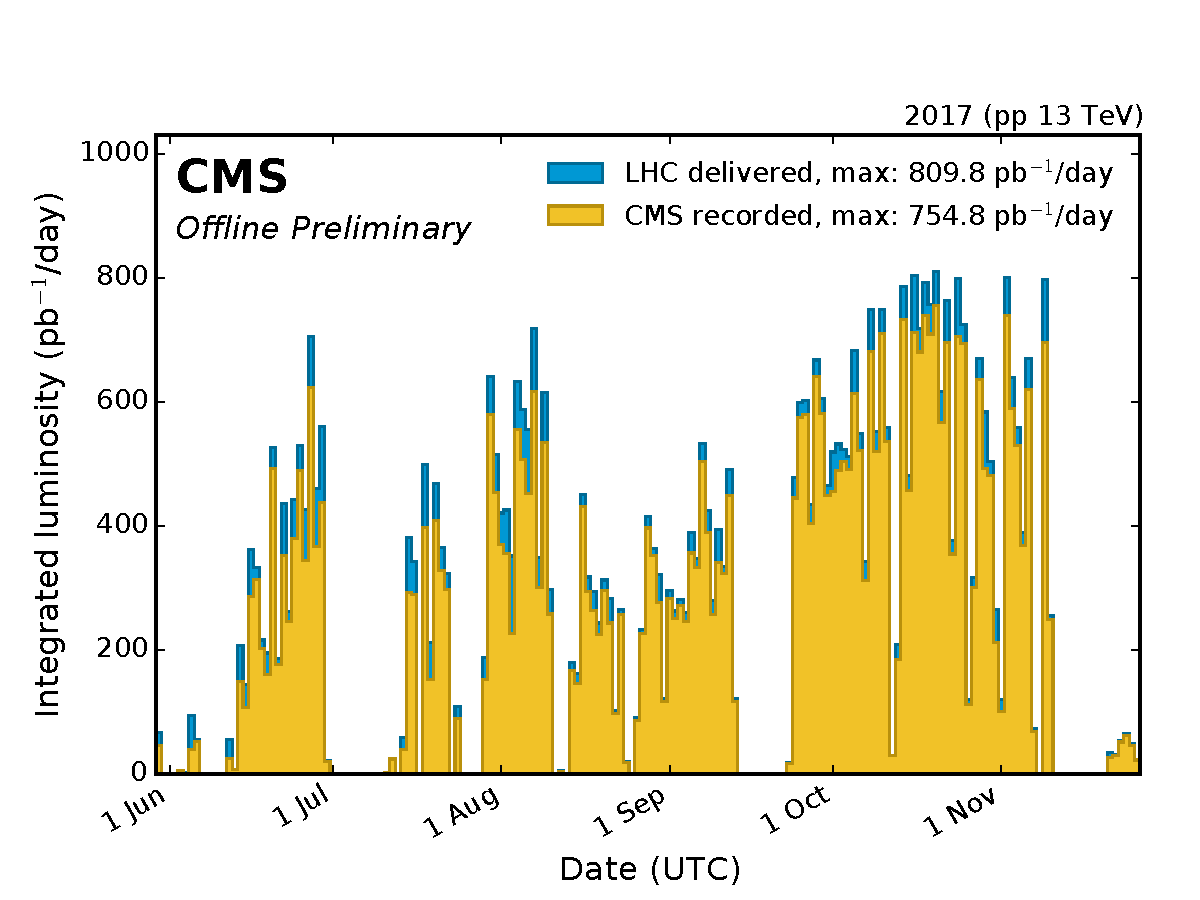
\includegraphics[width=.45\textwidth]{Chapter3/Luminosity/int_lumi_per_day_pp_2017_Normtag.pdf}
    \caption[Cumulative day-by-day integrated luminosity in 2017]{(left) Cumulative day by day integrated luminosity. (rigth) Day by day integrated luminosity, 2017 as the first plot, but not cumulative.} 
    \label{Lumi_2017}
  \end{figure}
\end{center}



\begin{center}
  \begin{figure}[h!]
    \centering
    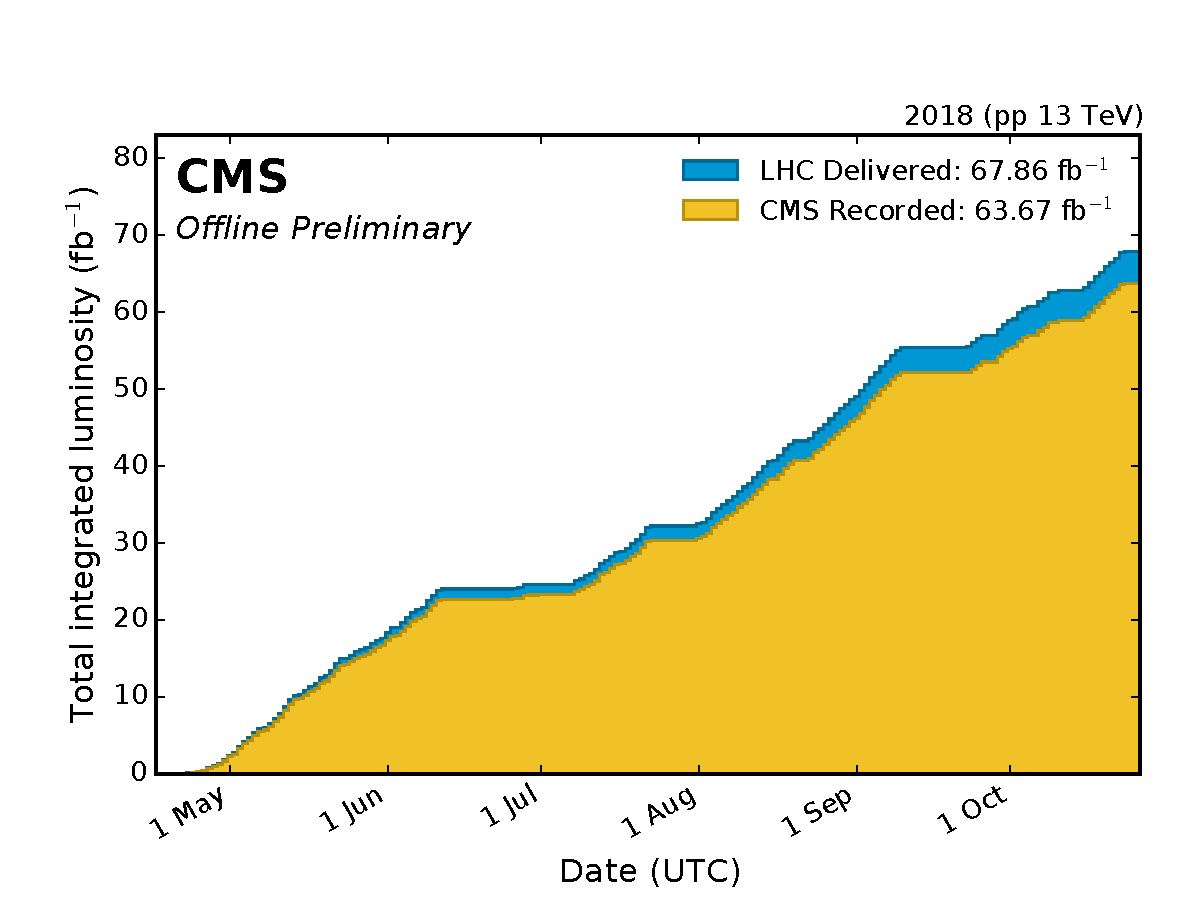
\includegraphics[width=.45\textwidth]{Chapter3/Luminosity/int_lumi_per_day_cumulative_pp_2018_Normtag.pdf}
    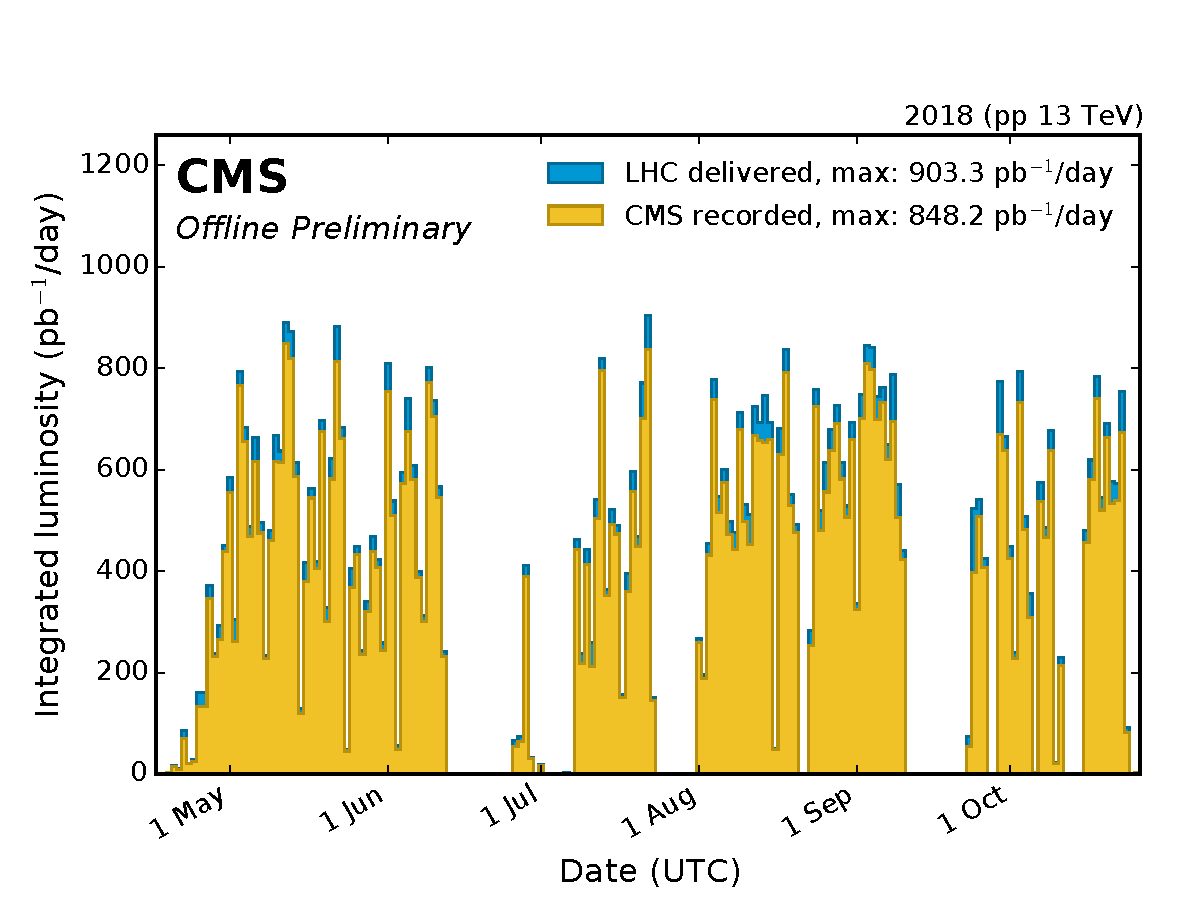
\includegraphics[width=.45\textwidth]{Chapter3/Luminosity/int_lumi_per_day_pp_2018_Normtag.pdf}
    \caption[Cumulative day-by-day integrated luminosity in 2022]{(left) Cumulative day by day integrated luminosity. (rigth) Day by day integrated luminosity, 2018 as the first plot, but not cumulative.} 
    \label{Lumi_2018}
  \end{figure}
\end{center}






\section{vdM program and Scan types}
\label{vdM program and Scan types}

Each year, the vdM scan program for the CMS experiment is conducted during specific LHC fills using a dedicated setup. The LHC filling schemes are designed with a specific number of bunch pairs at the CMS interaction point (IP5), for the especific case of 2017 an 2018 was at a proton-proton collision energy of \(\sqrt{s} = 13\) TeV. These scans play a crucial role in the precise determination of the luminosity by measuring the transverse beam profiles and overlap integral.  

To minimize long-range beam-beam effects and detector afterglow, the bunches are arranged in a way that optimizes the measurement conditions. During these special fills, the beams are systematically displaced in the transverse plane, allowing for a detailed study of beam dynamics and interaction rates. Various types of scan pairs with different characteristics were conducted to refine the accuracy of the luminosity determination.  

Each scan pair consisted of two scans in the transverse \(x\) and \(y\) planes. These included standard vdM scans, emittance scans, beam imaging scans, offset scans, and length scale calibration scans, each serving a specific purpose in the measurement process. A detailed description of each scan is provided below.  

\noindent \textbf{Standard vdM}: used specifically to compute $\sigma_{vis}$, in this scan the two beams are separated by $6\sigma_{b} \thickapprox 578\mu m$, where $\sigma_{b}$ represents the transverse bunch size. and scanned across each other in a se quence of 25 steps with 30 seconds per step with a step size of $0.5\sigma_{b} \thickapprox 48 \mu m$ in either the horizontal (x) or vertical (y) direction.\\

\noindent \textbf{Emittance}: same procedure as the standard vdM scans except the maximum separation (2.5 − 4σb), the number of steps (7 or 9) and the time per step (10 seconds) are smaller, so that the scan takes a shorter time. These type of scans are also performed in physics conditions as discussed in Section.\\
 
\noindent \textbf{Beam imaging}: in these scans, one beam (beam 1 and beam 2, respectively) is kept fixed at its nominal head-on position, while the other beam is separated and scanned in 19 steps, each step lasts 46 seconds and covers a range from $-4.5\sigma_{b}$ to $+4.5\sigma_{b} \thickapprox 433 \mu m$. These scans were developed for studies on beam shapes, estimating the uncertainty caused by the correction called $x$-$y$ non-factorization described in the next chapter. BI scans are also analyzed as traditional vdM scans and used to compute of $\sigma_{vis}$.\\
 
\noindent \textbf{Constant-Separation Length Scale}: during this scan the two beams are separated by $\sqrt{2} \sigma_{b} \thickapprox 106 \mu m$ (approximately equal to $1 \Sigma_{b}$) and moved together in steps of $1\sigma_{b}$ forward and backward in five steps each, for a total of 10 steps with 70 seconds per step.\\

\noindent \textbf{Variable-Separation length scale}: one beam (starting with beam 1) is moved to $-2.5\sigma_{b}$ and then a three-point scan is performed with the other beam (starting with beam 2) at arelative position of $+-1.25\sigma_{b}$, 0, and $+1.25\sigma_{b}$. The position of the first beam is then stepped in five steps to $+2.5\sigma_{b}$, repeating the three-point scan (“miniscan”) at each step. This procedure is repeated four times, with two directions for each of the two beams. Each scan point has a duration of about 46 s.
 
The two types of Length scale are pecial scan designed to apply a correction to the results of  $\sigma_{vis}$ obtained from the vdM scan program, this correction will be described further in this section.\\
 
\noindent \textbf{Offset}: same procedure as the standard vdM scans except that the beams are separated by  range from $-3\sigma_{b}$ to $+3\sigma_{b}$ in the non-scanning direction.\\ 
 
\noindent \textbf{Super Separation}: this type of scan is performed for background estimation. In this scan, the two beams are separated by a distance of \(6\sigma_{b}\) for 5 minutes. At this distance, the beam overlap is minimal, and the contribution from collisions is negligible.  
There can be more than one Super Separation scan per scan program, this is useful to understanding the behavior of the background throughout the year and for subtracting it accordingly.

The data collected from these scans provide the essential input for luminosity calibration, which is critical for cross-section measurements and precision physics analyses at the LHC.
 
\subsection{2017 vdM scan program}
\label{2017 vdM scan program}

The 2017 vdM scan program was performed during LHC fill 6016 on 28 July 2017, at a center-of-mass energy of 13 TeV. The LHC filling scheme included 32 colliding bunch pairs at the CMS interaction point (IP5). In the special case of PCC, to ensure a dataset with a high event count at large beam separations, CMS gated the zero-bias triggers on 5 bunch pairs (BCIDs 41, 281, 872, 1783, and 2063) and recorded events at a total rate of 18 kHz.  

The bunch intensities were approximately \(9 \times 10^{10}\) protons per filled bunch, resulting in a total beam intensity of approximately \(4.5 \times 10^{12}\) protons per beam. The total beam intensities were measured with the DC Current Transformers (DCCT) ~\citep{LHC_DCCT_calibration}.  The beam orbit was monitored using two systems: the DOROS beam position monitors (BPMs) ~\citep{BPM__electronics}, located near IP5, and the arc BPMs, located in the LHC arcs adjacent to CMS.  

The vdM scan program consisted of a total of eight orthogonal (x-y) scan pairs. It started with a short emittance scan, em1. Four scans were standard vdM scans: vdM1 (2), vdM3 (6), and vdM4 (11). These scans were performed first in the x direction and then in the y direction. The intermediate scan, vdM2 (3), was performed first in the y direction and then in the x direction. This was done to check reproducibility.  

Two scan pairs of beam imaging scans were performed, with beam 1 and beam 2 scanning. Pairs Im1 and Im2 corresponded to scans 4 and 5, respectively. Scan pair 7 was an offset scan (off) performed just after vdM3, but it is not used in this analysis.  

A length scale calibration (LSC) program was performed at the end of the vdM program using two different LS methods. The first method was the constant-separation scan (cLS), performed as scan 8 in this program. This type of scan had been previously used in the 2015–2016 publication  ~\citep{lumi_precise_2015_2016} for the CMS length scale calibration.

The second method consisted of variable-separation scans, vLS1 and vLS2, which were scans 9 and 10, respectively, in the LS program. This method was used for the first time in 2017, following the scan protocol originally developed by ATLAS.  

The top of Figure~\ref{BeamPosition_2017} shows the beam positions for the two beams in the x and y directions as measured by the DOROS BPMs during the 2017 scan program, showing the four regular scan pairs, the two beam imaging scan pairs, the offset scan pair, and the two length scale scan programs, with the abbreviations used for the scans introduced.  

%\begin{center}
  \begin{figure}[h]
    \hspace{-.4cm}
    %\centering
    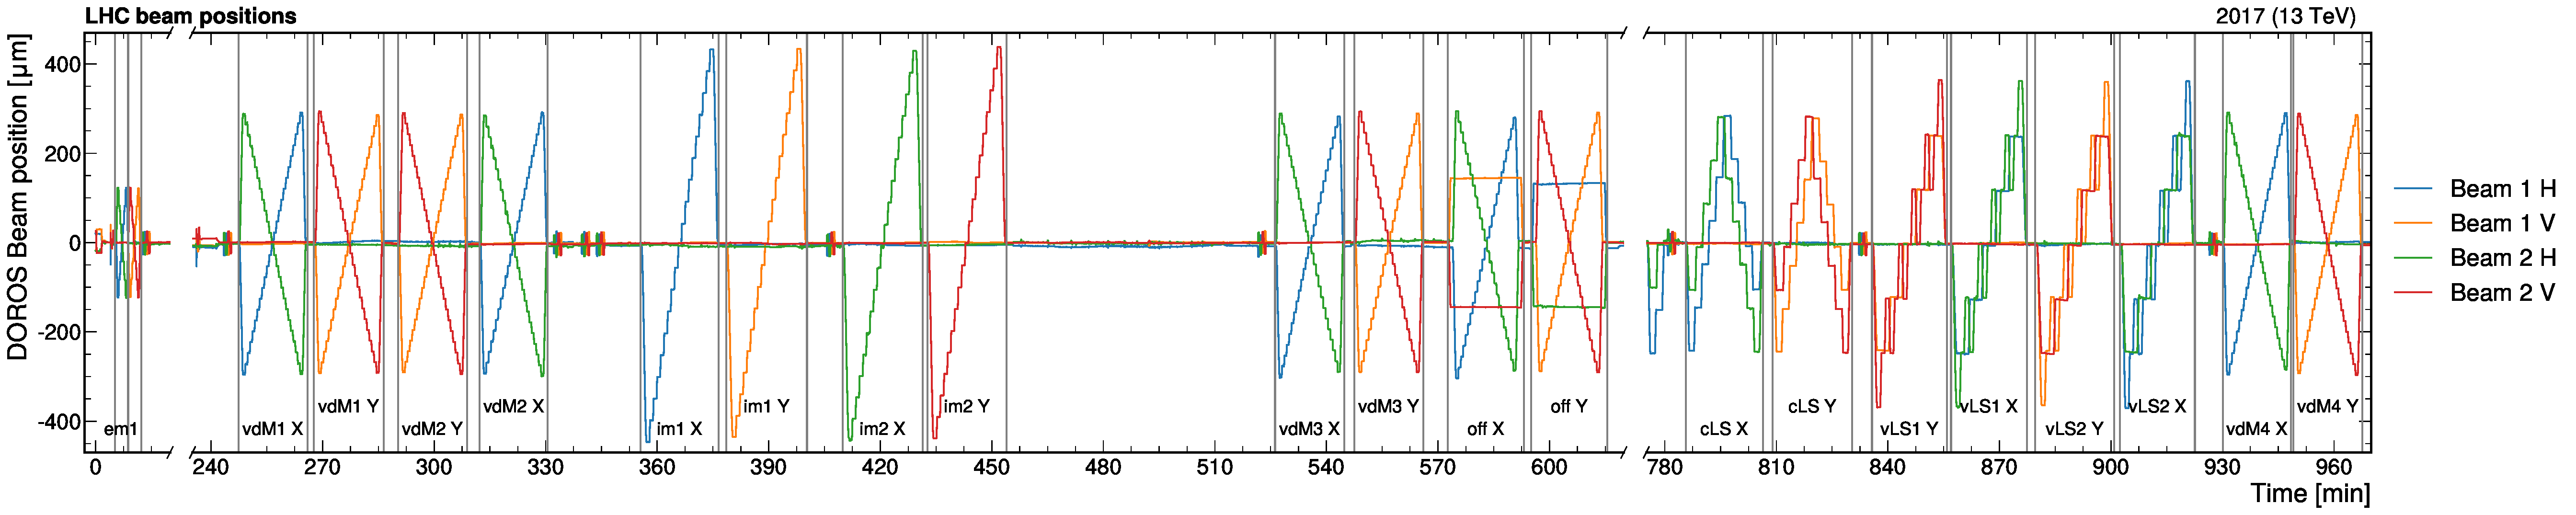
\includegraphics[scale=.17]{Chapter3/BeamPosition/doros_vs_time_6016.pdf}
    \caption[Doros]{ Vertical (V) and horizontal (H) beam positions as a function of time measured by the DOROS beam position monitors during LHC fill 6016. The orbit is averaged over the bunches and monitored throughout the scan program with 1 second time granularity. The individual scans are delimited by the vertical lines. Each scan pair consists of two scans orthogonal to each other and labelled with the abbreviation of the specific scan type}
    \label{BeamPosition_2017}
  \end{figure}
%\end{center}


\subsection{2018 vdM scan program}
\label{2018 vdM scan program}

The 2018 vdM scan program was conducted during LHC fill 6868 from June 30 to July 1, 2018, at a center-of-mass energy of 13 TeV. The LHC filling scheme included 124 colliding bunch pairs at the CMS interaction point (IP5). For the special case of PCC, to ensure a dataset with a high event count at large beam separations, CMS gated the zero-bias triggers on 5 bunch pairs (BCIDs 265, 865, 1780, 2192, and 3380) and recorded events at a total rate of 27 kHz.  

The bunch intensities were approximately \(7-9 \times 10^{10}\) protons per filled bunch, resulting in a total beam intensity of approximately \(4.5 \times 10^{13}\) protons per beam. The total beam intensities were measured with the DC Current Transformers (DCCT) ~\citep{LHC_DCCT_calibration}.  The beam orbit was monitored using two systems: the DOROS beam position monitors (BPMs) ~\citep{BPM__electronics}, located near IP5, and the arc BPMs, located in the LHC arcs adjacent to CMS.  

The vdM scan program was conducted in two parts due to an alarm and a power cut. The first part consisted of a total of five x-y scan pairs.First, two short emittance scans, em1 (1) and em2 (2), were conducted, respectively. Then, a standard vdM scan pair, vdM1 (3), was performed, followed by an offset scan, off1 (4). Finally, a pair of beam imaging scans, BI1 (5) and BI2 (6), were onducted, but only the first was completed before the alarm interrupted the program.  

The second part of the program was conducted approximately 7.5 hours later and consisted of 12 scan pairs. Scan pair em3 (6) was a short emittance scan, followed by beam imaging scan pairs Im3 (7) and Im4 (8), then an offset scan pair, off2 (9), and finally two standard vdM scan pairs, vdM2 (10) and vdM3 (11). The latter two allowed us to test the reproducibility of the measurement.  

A length scale calibration program was performed after vdM3 using constant-separation and variable-separation scan pairs: cLS (12), vLS1 (13), and vLS2 (14). Finally, a standard vdM scan pair, vdM4 (15), and two short emittance scan pairs, em4 (16) and em5 (17), concluded the program.  

In each scan pair, the scan was performed first in the x direction and then in the y direction, with the exception of the variable vLS calibration scan pairs, which were performed in the opposite order.  

Additionally, two Super Separation periods were conducted. The first, SS1, took place right after vdM3 was completed, and the second, SS2, followed vdM4. These periods are not included in the final count of scan pairs since they only involve separating the beams in a single direction. They are used for the final estimation of background noise, which will be subtracted in the final analysis. The details of these periods will be discussed in the following chapter.  

The bottom of Figure~\ref{BeamPosition_2018} shows the beam positions for the two beams in the x and y directions as measured by the DOROS BPMs during the 2018 scan program, showing the 17 scan pairs.4 regular scan pairs, the 3 beam imaging scan pairs, the 2 offset scan pair, and the 3 length scales, the emitance scan a the 2 Superseparation periods with the corrsponding abbreviations used.  


%[15] M. Gasior, J. Olexa, and R. Steinhagen, “BPM electronics based on compensated diode detectors — results from development systems”, Conf. Proc. C1204151 (2012) 44.
%[7] C. Barschel et al., “Results of the LHC DCCT calibration studies”, Technical Report 2349 CERN-ATS-Note-2012-026 PERF, 2012.


%\begin{center}
  \begin{figure}[h]
  \hspace{-0.4cm}
    %\centering
    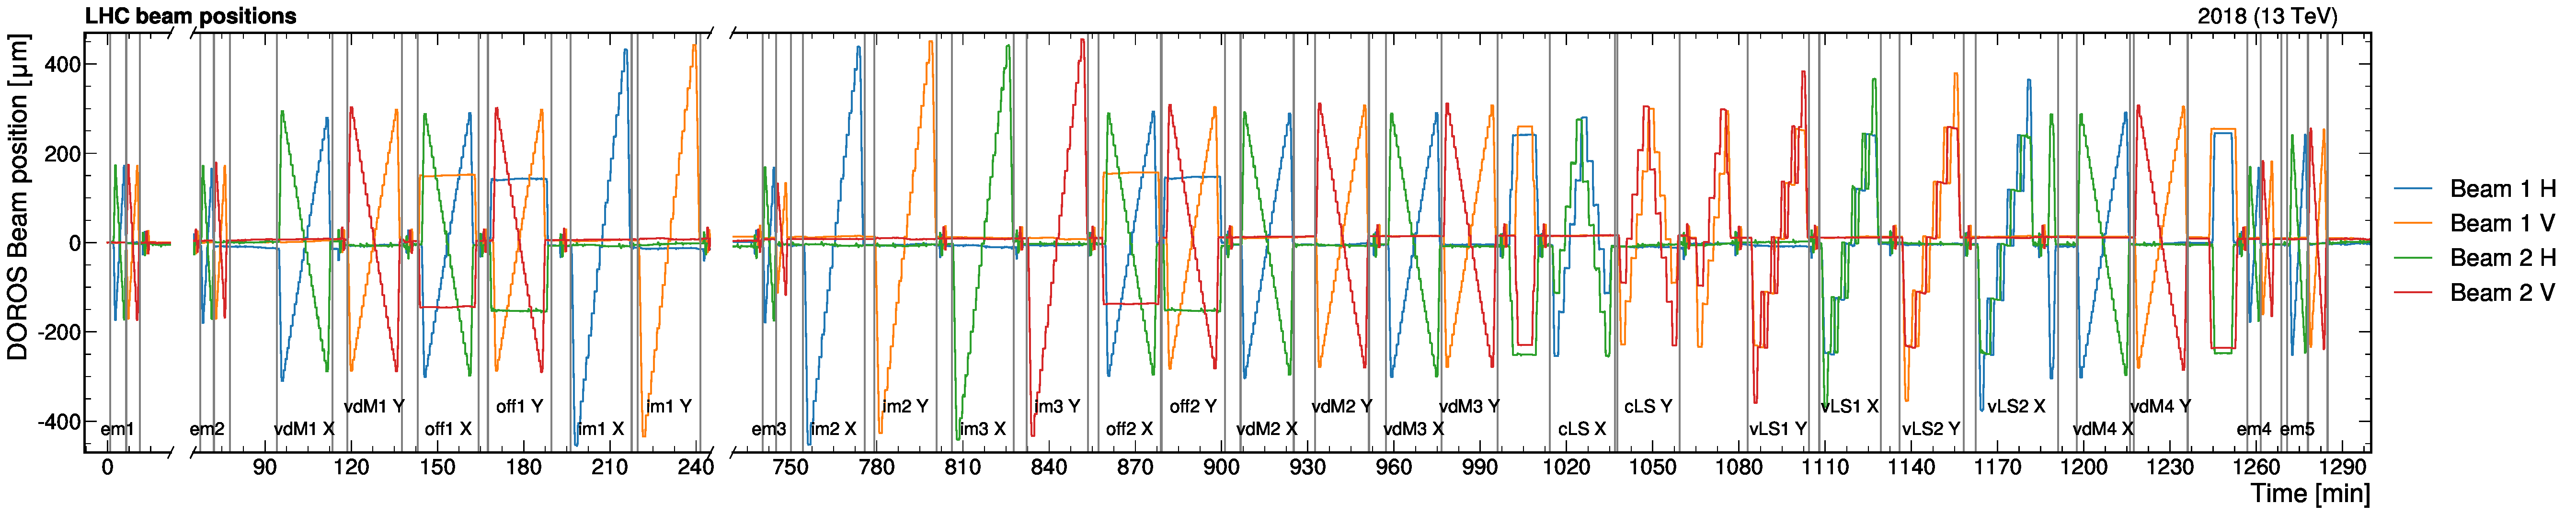
\includegraphics[scale=.17]{Chapter3/BeamPosition/doros_vs_time_6868.pdf}
    \caption[Doros]{Vertical (V) and horizontal (H) beam positions as a function of time measured by the DOROS beam position monitors during LHC fill 6868. The orbit is averaged over the bunches and monitored throughout the scan program with 1 second time granularity. The individual scans are delimited by the vertical lines. Each scan pair consists of two scans orthogonal to each other and labelled with the abbreviation of the specific scan type.}
    \label{BeamPosition_2018}
  \end{figure}
%\end{center}


